\documentclass[a4paper,10pt]{article}
\usepackage{anysize}
\usepackage{amsmath}
\usepackage{amssymb}
\usepackage{graphicx}
\usepackage[left=0.75in, right=0.75in, top=0.5in, bottom=0.75in, includefoot, headheight=13.6pt]{geometry}
\usepackage{color,graphicx}
\usepackage{verbatim}
\usepackage{hyperref}
\usepackage{multirow}
\usepackage{latexsym}
\usepackage{mdwlist}
\usepackage{tabularx}

\renewcommand{\labelitemii}{$\circ$}



\hypersetup{
    bookmarks=true,         % show bookmarks bar?
    unicode=false,          % non-Latin characters in Acrobat's bookmarks
    pdftoolbar=true,        % show Acrobat's toolbar?
    pdfmenubar=true,        % show Acrobat's menu?
    pdffitwindow=true,      % page fit to window when opened
    pdftitle={CV},    % title
    pdfauthor={Gunjan},     % author
    pdfsubject={Placements},   % subject of the document
    colorlinks=true,       % false: boxed links; true: colored links
    linkcolor=magenta,        % color of internal links
    citecolor=blue,        % color of links to bibliography
    filecolor=magenta,      % color of file links
    urlcolor=black           % color of external links
}

% Margines

\addtolength{\oddsidemargin}{-0.215in}
\addtolength{\textwidth}{0.2in}

\definecolor{titleColor}{rgb}{0.631, 0.776, 0.925}

\begin{document}

%%%%%%%%% virtical space %%%%%%%%%%%%%%%%%


\begin{table}[h!]
  \begin{center}
    \begin{tabular}{  l  p{10cm}  p{8cm}}
      \raisebox{-\totalheight}{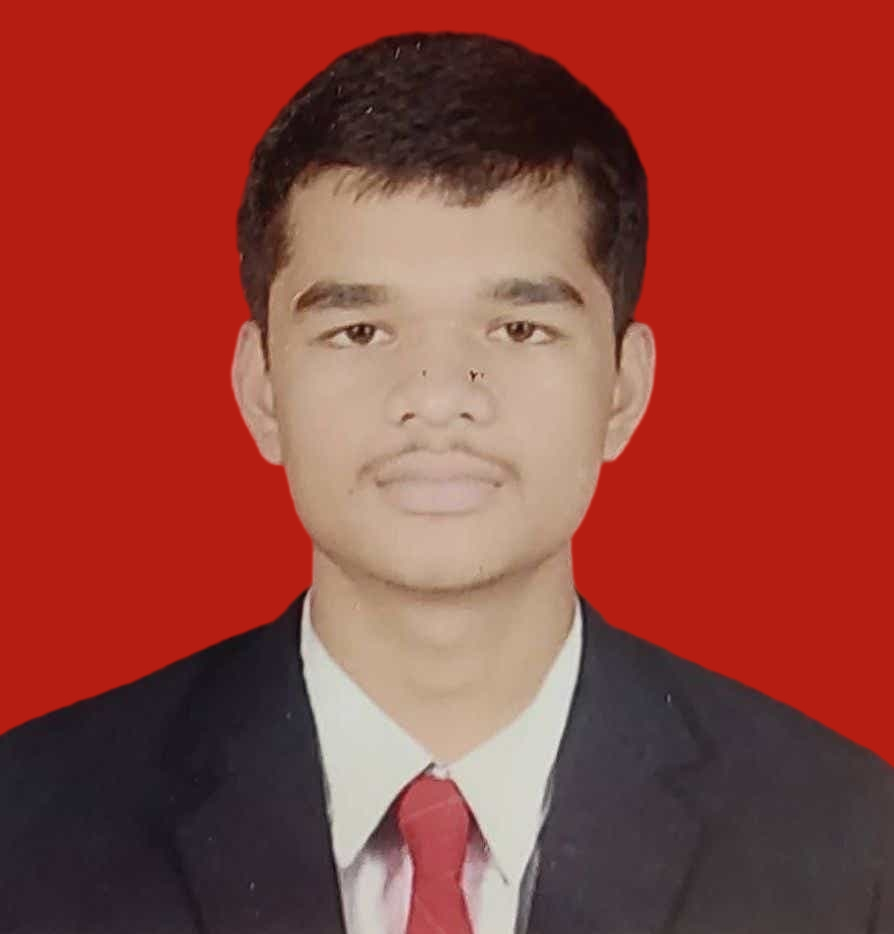
\includegraphics[scale=.075]{gunjan}}
       &
      \begin{itemize}
        \setlength\itemsep{.01em}
        \item[] \textbf{Gunjan Atul Lunkad}
        \item[] \textbf{\href{mailto:glunkad26@gmail.com}{glunkad26@gmail.com}}
        \item[] \textbf{\url{http://www.linkedin.com/in/gl-gunjan-lunkad}}
        \item[] \textbf{\url{http://github.com/glunkad}}
      \end{itemize}
       &
      \begin{itemize}
        \setlength\itemsep{.01em}
        \item[] \textbf{Male}
        \item[] \textbf{DOB: 26/01/2001}
        \item[] \textbf{+91 7620980424}
      \end{itemize}
    \end{tabular}
  \end{center}
\end{table}

\vspace{-.8cm}

\begin{tabularx}{.98\textwidth}{llp{2cm}lll}
  \hline
  \textbf{Examination} & \textbf{Specialization}          &  & \textbf{University / Board} & \textbf{Year} & \textbf{CPI} \\
  \hline
  Graduation           & Electronics \& Telecommunication &  & PCCOE                       & 2023          & 8.24/10      \\
  Intermediate         & -                                &  & HSC                         & 2019          & 69.8/100     \\
  Matriculation        & -                                &  & SSC                         & 2017          & 87.6/100     \\
  \hline
\end{tabularx}
\\\\

%{\qquad \\ \\ \\ \\ \\ \\ \\ \\ \\ \\ \\ \\ \\}

\colorbox{titleColor}{\parbox{6.7in}{\textbf{INTERNSHIP}}}
\begin{itemize}
  \setlength{\itemsep}{1pt}
  \item {{Computer Architecture, Multi-core Architecture, Embedded Systems, Signal Processing}}
\end{itemize}

\colorbox{titleColor}{\parbox{6.7in}{\textbf{Technical Proficiency}}}\\

\begin{tabular}{p{1.6in}p{0.1in}p{4.5in}}
  \textbf{\small{Operating Systems}}     & : & {{Windows, Linux}}                                                      \\
  \textbf{\small{Programming Languages}} & : & {{C, Python, C++, VHDL, Verilog}}                                       \\
  \textbf{\small{Hardware Platforms}}    & : & {{8051, 8086, ATMEL AVR, Altera EPM3064, MaxV 5M1270 CPLDs}}            \\
  \textbf{\small{Softwares/Tools}}       & : & {{Sniper, McPAT, PinPoints, MATLAB, TortoiseHg, Visual Studio, \LaTeX}} \\
\end{tabular}


\colorbox{titleColor}{\parbox{6.7in}{\textbf{Key Academic Projects}}}

\begin{itemize*}
  \setlength{\itemsep}{1pt}
  \item \textbf{M.Tech Thesis - Scheduling Heterogeneous Multi-cores: Using Performance Variation Across Phases}  \\
  {(Guide : Prof. Virendra Singh, IIT Bombay)} \hfill {\small{{\textbf{[Jul '13 - Jul '14]}}\/}}
  \begin{itemize*}
    \setlength{\itemsep}{.00pt}
    \item \textbf{Abstract}: In the multicore era apart from the challenge of increasing processor's performance, computer architects must also focus on designing energy efficient multicore processor so that processor's power consumption doesn't exceed its power budget. A dynamic scheduler was proposed which analysed the performance variation of an application at runtime to utilize time-varying execution behaviour of the application and schedules the application on the most suitable idle core among all the cores available in heterogeneous multi-core architecture. The work compared a static scheduler with the dynamic scheduler. It was shown that the dynamic scheduler is more power efficient than static scheduler with an average perf/watt benefit of 26\% on the analysed benchmarks.

  \end{itemize*}
\end{itemize*}

\begin{itemize*}
  \setlength{\itemsep}{1pt}
  \item \textbf{R\&D Project - Opportunities and Challenges in Multicore Architecture} \\
  {(Guide : Prof. Virendra Singh, IIT Bombay)}  \hfill {\small{{\textbf{[Jan '13 - Jun '13]}}\/}}
  \begin{itemize*}

    \setlength{\itemsep}{.00pt}
    \item \textbf{Abstract} Migration from single-core to many-core era has provided us with various opportunities \& challenges. Reviewed literature related to different core configurations like homogeneous, heterogeneous \& morphcores and analysed the challenges in designing a computer architecture in constrained power budget.
  \end{itemize*}
\end{itemize*}


\colorbox{titleColor}{\parbox{6.7in}{\textbf{ Relevant Technical Projects}}}

\begin{itemize*}
  \setlength{\itemsep}{1pt}
  \item \textbf{\small{Implementation of Cache Replacement Policies}} \hfill {\small{{\textbf{[Mar '13 - Apr '13]}}}\/}
  \begin{itemize*}
    \item Implemented LLC Cache Replacement Policies like LRU, LFU, SRRIP, DRRIP, ABRip.
  \end{itemize*}
\end{itemize*}

\begin{itemize*}
  \setlength{\itemsep}{1pt}
  \item \textbf{\small{Design of 2 way Out of Order (OoO) Superscalar ARM 7 Processor}} \hfill {\small{{\textbf{[Mar '13 - Apr '13]}}}\/}
  \begin{itemize*}
    \item Studied ARM ISA \& developed the required control words and designed necessary processor architecture.
    \item Implemented using Verilog, major hardware blocks like Branch Predictor, Instruction Decoder, Reservation Station, 5 Stage Pipeline, ROB etc. required for out of order execution of instruction.
  \end{itemize*}
\end{itemize*}

%\begin{itemize*}
%  \setlength{\itemsep}{1pt}
%  \item \textbf{\small{Developed level 2 hardware flowchart for 8085 ISA}} \hfill {\small{{\textbf{[Feb '11 - March '11]}}}\/} 
%\begin{itemize*}
%	\item Developed level 2 flowchart for each instruction, designed control word and suitable datapath and controller.
%\end{itemize*}
%\end{itemize*}

%\begin{itemize*}
%  \setlength{\itemsep}{1pt}
%  \item \textbf{\small{Automatic Seed Sowing Bot for Green House}} \hfill {\small{{\textbf{[Sep '12 - Nov '12]}}}\/} 
%\begin{itemize*}
%	\item Aim of the project was to design a prototype to automate the seed sowing process in a green house. User should choose the trough number in the Green House through a GUI located remotely. 
%	\item The bot moves to the location of the choosen trough without manual intervention and sows the seeds at appropriate interseeding distances.
%\end{itemize*}
%\end{itemize*}

\begin{itemize*}
  \setlength{\itemsep}{1pt}
  \item \textbf{\small{Interrupt Controller of Microprocessor 8085}} \hfill {\small{{\textbf{[Apr '12]}}}\/}
  \begin{itemize*}
    \item Hardware and software interrupts were implemented using VHDL.
    \item Synchronisation, timing constraints,
    \& handshaking with other internal modules were taken care of.
  \end{itemize*}
\end{itemize*}

\begin{itemize*}
  \setlength{\itemsep}{1pt}
  \item \textbf{\small{Data Processor of Microprocessor 8085}} \hfill {\small{{\textbf{[Mar '12]}}}\/}
  \begin{itemize*}
    \item All data movement and ALU operation instruction were implemented using Verilog.
    \item Handshaking with Bus Interface Unit was also implemented for memory read/write operations.
  \end{itemize*}
\end{itemize*}

\colorbox{titleColor}{\parbox{6.7in}{\textbf{Work Experience}}}


\begin{itemize*}
  \setlength{\itemsep}{.00pt}
  \item \textbf{{Senior Software Engineer, Huawei Technologies India Pvt. Ltd., Bangalore}} \hfill {\small{{\textbf{[Jun '08 - Jul '11]}}\/}}
  \begin{itemize*}
    \item \textbf{Development of MDBLite: Database to store messages in mobile phones}.\\
    Being part of the platform team, developed APIs to provide services to the application (GUI) team. Responsible for development of APIs, their functionality testing, release activities and later maintenance of the project. C language was used on BREW platform for the development of interfaces.
  \end{itemize*}
  \begin{itemize*}
    \item \textbf{Development of RSS Reader for Smartphones.}\\
    Understood the already developed module and customized it to support new feature requirements for the smartphones. Responsible in increasing the speed of the app by changing the database structure which was used to store the content of the RSS feeds in the SQLite DB. Added new feature to update the RSS feeds automatically as per user setting.
  \end{itemize*}
  \begin{itemize*}
    \item \textbf{Development of GUI for Conversation and Panchang App for Smartphone}.\\
    Developed Graphical User Interface for Conversation (SMS app) and Panchang (Vedic Astrology app)
  \end{itemize*}
\end{itemize*}

\begin{itemize*}
  \setlength{\itemsep}{.00pt}
  \item \textbf{{Research Assistant, Wadhwani Electronics Lab, IIT Bombay}} \hfill {\small{{\textbf{[Jul '11 - Jul '14]}}\/}} \\
  {(Guide : Prof. Mahesh B. Patil, IIT Bombay)}
  \begin{itemize*}
    \item Working as a Teaching Assistant for conducting undergraduate lab courses.
  \end{itemize*}
  \begin{itemize*}
    \item Conducted workshops on Modern Digital Design at BVM Engineering College, Vallabh Vidyanagar, Anand, Gujarat as part of e-Prayog, ``Virtual Labs", IIT Bombay, an MHRD initiative.
  \end{itemize*}
\end{itemize*}


%\begin{itemize*}
%  \setlength{\itemsep}{1pt}
%  \item \textbf{\small{M.Tech Seminar: Review of Methods of Speech Synthesis}} \hfill {\small{{\textbf{[Jun '11 - Nov '11]}}}\/} 
%\begin{itemize*}
%	\item Speech synthesis is the technique of converting given input text to synthetic speech.
%	\item A comprehensive literature review of majorly researched methods of speech synthesis was done.
%\end{itemize*}
%\end{itemize*}

%\begin{itemize*}
%  \setlength{\itemsep}{1pt}
%  \item \textbf{\small{An aid in communication for the mute}} \hfill {\small{{\textbf{[Aug '12 - Jan '13]}}}\/} 
%\begin{itemize*}
%	\item Project proposal selected for Texas Instruments(TI) analog design contest 2012.
%	\item Going to design a portable unit for the mute person which generates speech equivalent of his hand gestures.
%	\item Right now, we are working upon the 1st part of analog design contest i.e., simulation of 2nd order LPF using TL082
%         op-amp.
%\end{itemize*}
%\end{itemize*}

%\begin{itemize*}
%  \setlength{\itemsep}{1pt}
%  \item \textbf{\small{Discrete Logarithm Problem}} \hfill {\small{{\textbf{[Jan '12 -  May '13]}}}\/} 
%\begin{itemize*}
%	\item Implemented the BSGS method for solving DL problem for an extension field of prime 3 i.e., $3^m$ in SAGE.
%	\item Value is found upto 8 digits of input, and m is varied from 1 to 25.
%\end{itemize*}
%\end{itemize*}

\colorbox{titleColor}{\parbox{6.7in}{\textbf{Relevant Courses}}}\\[0.08in]
\begin{tabular}{p{3.5in}p{3in}p{2.5in}}
  \hspace{0.9pc}$\bullet$ Processor Design                         & $\bullet$ Embedded Systems Design \\[0.05in]
  \hspace{0.9pc}$\bullet$ Advanced Computer Archiecture            & $\bullet$ Embedded Systems        \\[0.05in]
  \hspace{0.9pc}$\bullet$ Advanced Topics in Computer Architecture & $\bullet$ VLSI Design Lab         \\[0.05in]
\end{tabular}
\\\\
\colorbox{titleColor}{\parbox{6.7in}{\textbf{Scholastic Achievements}}}\\
\begin{itemize}
  \setlength{\itemsep}{1pt}
  \item Recipient of \textbf{Research Assistant Scholarship} at Indian Institute of Technology Bombay by Ministry of Human
        Resource Development, Government of India
  \item \textbf{Dean's Appreciation Letter} from Faculty Coordinator, Student Mentor Program; Dean, Student Affairs and Dean,
        Academic Program, IIT Bombay for remarkable efforts on student mentoring of post graduate students as the overall coordinator of Institute Student Companion Program, IIT Bombay.
\end{itemize}

\colorbox{titleColor}{\parbox{6.7in}{\textbf{Positions of Responsibility}}}\\

\textbf{Overall-Coordinator, Institute Student Companion Programme (ISCP)}  \hfill {\small{{\textbf{[May '13 - April '14]}}}\/}
\begin{itemize*}
  \item Leading the ISCP team in creating an environment for smooth transition of PG freshers to the new college.
  \item Selected a team of 140 mentors to guide, help and motivate PG freshers in pursuit of their academic and non-academic goals. Working with the team in organising Orientation Programs, Workshops and session for freshers.
  \item Around 80\% freshers found that the allotted mentors and programs done by ISCP were very helpful.

\end{itemize*}

%\textbf{PG Coordinator, Robotics Club, STAB} \hfill {\small{{\textbf{[Jul '12 - Apr '13]}}}\/} 
%\begin{itemize*}
% \item Responsible for increasing PG participation in institute level technical activities.
%% \item Organised ROFL (Research Only for Fun) event for PG students.
% \item Selected as the Best PG Coordinator for my contribution to the club.
%\end{itemize*}

%\textbf{Techical Secretary, H14, IIT Bombay} \hfill {\small{{\textbf{[Jul '12 - Apr '13]}}}\/} 
%\begin{itemize*}
% \item Ensured adequate hostel representation in institute level technical activities.
%\end{itemize*}

%\textbf{Committee Head, Certificate and Memento, Confluence'08, NIT Kurushetra} 
%\begin{itemize*}
% \item Managed the preparation and distribtution of certificates and mementos in Confluence'08.
%\end{itemize*}

\colorbox{titleColor}{\parbox{6.7in}{\textbf{Extra Curricular activities}}}

\begin{itemize}
  \setlength{\itemsep}{1pt}
  %  \item Best Team in "Paisa Parliament Policy", a simulation game competition organised by ShARE IITB.\hfill {\small{{[Aug '13]}}\/} 
  \item Part of the team of 937 students which was awarded \textbf{Guinness World Record} and \textbf{Limca Book of Record} for solving 3   x 3 x 3 Rubik Cube puzzle with most students at a time. \hfill {\small{{[Mar '12]}}\/}
  \item Secured \textbf{First} position in E-Modelling and Kritika (circuit designing contest) in APEX'06, POWERFEST'07 (National Level Techical Fest) at NIT Kurukshetra. \hfill {\small{{[Nov '06, Feb '07]}}\/}
        %  \item Wrote Best Poem titled "Mata-Pita" (Mother-Father) in Kavita Lekhan in Hindi Saptaah (Week) at NITK.  
\end{itemize}

\colorbox{titleColor}{\parbox{6.7in}{\textbf{Hobbies and Interests}}}
%\vspace{0.5 pt}

\begin{itemize}
  \setlength{\itemsep}{1pt}
  \item Watching Documentaries, Reading Fiction and Non-Fiction books, Trekking, Solving Rubik Cube
\end{itemize}

\textit{Updated on 26th Dec 2016}
\end{document}

